%! Author = chtompki
%! Date = 1/14/26
% Example LaTeX document for GP111 - note % sign indicates a comment
\documentclass[12pt]{amsart}
% Default margins are too wide all the way around. I reset them here
\setlength{\hoffset}{-.75in}
\setlength{\textwidth}{6.5in}
\setlength{\voffset}{-.5in}
\setlength{\textheight}{9.0in}
\usepackage{amsmath}
\usepackage{amssymb}
\usepackage{amsthm}
\usepackage{pgfplots}
\usepackage{enumerate}
\usepackage{tikz}
\usetikzlibrary{shadows,arrows,arrows.meta,shapes,positioning,calc}% Required for the Circle and Triangle arrow tips
\usepackage{setspace}
\usepackage{siunitx}

\theoremstyle{conjecture}
\newtheorem{conjecture}{Conjecture}

\theoremstyle{definition}
\newtheorem{definition}{Definition}

\theoremstyle{question}
\newtheorem{question}{Question}

\theoremstyle{theorem}
\newtheorem{theorem}{Theorem}

\title{Seminar Summary:\\April 28, 2026 - Glenn Hurlbert\\Graph Pebbling}
\author{Rob Tompkins}
\date{\today}


\begin{document}
    \maketitle
    \date{\today}
    \begin{onehalfspace}
        \begin{figure}
            \begin{tikzpicture}[
                scale=1.05,
                v/.style={circle, fill=black, inner sep=2pt},
                peb/.style={circle, draw, thick, fill=white, inner sep=7pt, font=\large},
                lab/.style={font=\large}
            ]

% vertices
                \node[v] (a) at (0,0) {};
                \node[v] (b) at (0,1.2) {};
                \node[v] (c) at (0.9,2.15) {};
                \node[v] (d) at (1.7,1.2) {};
                \node[v] (e) at (1.8,-1.0) {};

                \node[v] (f) at (2.9,-1.0) {};
                \node[v] (g) at (2.9,0) {};
                \node[v] (h) at (3.75,1.2) {};
                \node[v] (i) at (3.75,-1.0) {};
                \node[v] (j) at (3.65,2.25) {};

                \node[v] (k) at (5.7,2.25) {};
                \node[v] (l) at (5.8,1.2) {};
                \node[v] (m) at (5.8,0) {};

                \node[v] (n) at (7.7,1.2) {};
                \node[v] (o) at (7.7,-1.0) {};
                \node[v] (p) at (9.3,0) {};

% edges
                \draw (a)--(b)--(c)--(j)--(k);
                \draw (a)--(g)--(m)--(p);
                \draw (b)--(d)--(h)--(l)--(n);
                \draw (c)--(d);
                \draw (d)--(e)--(f)--(i)--(o);
                \draw (f)--(g)--(h)--(j);
                \draw (g)--(h);
                \draw (h)--(i);
                \draw (k)--(l)--(m);
                \draw (n)--(o);
                \draw (n)--(p)--(o);

% labels
                \node[peb] at (-0.45,1.2) {1};
                \node[peb] at (6.15,2.45) {2};
                \node[peb] at (7.75,-1.35) {5};

                \node[lab] at (2.55,0.25) {1};
                \node[lab] at (3.95,1.45) {15};
                \node[lab] at (5.95,0.25) {11};
                \node[lab] at (7.75,1.55) {5};
                \node[lab] at (1.45,-1.45) {3};

            \end{tikzpicture}
            \label{graphWithConfiguration}
            \caption{A graph with configuration}
        \end{figure}

        \begin{tikzpicture}[
            scale=1.1,
            every node/.style={circle, fill=black, inner sep=1.8pt},
            label/.style={circle, draw, fill=white, inner sep=4pt, font=\large}
        ]

% vertices
            \node (a) at (0,0) {};
            \node (b) at (0,1) {};
            \node (c) at (0.8,1.7) {};
            \node (d) at (1.5,1.1) {};
            \node (e) at (1.5,0.1) {};
            \node (f) at (1.5,-1.0) {};
            \node (g) at (2.7,-1.0) {};
            \node (h) at (2.7,0.4) {};
            \node (i) at (2.7,1.7) {};
            \node (j) at (3.9,2.2) {};
            \node (k) at (4.3,1.2) {};
            \node (l) at (4.3,0.4) {};
            \node (m) at (3.9,-0.6) {};
            \node (n) at (5.4,0.0) {};
            \node (o) at (5.4,1.6) {};
            \node (p) at (6.5,1.8) {};
            \node (q) at (6.5,0.3) {};
            \node (r) at (7.7,0.4) {};

% edges
            \draw (a)--(b)--(c)--(d)--(e)--(a);
            \draw (c)--(i)--(j)--(k)--(d);
            \draw (e)--(f)--(g)--(h)--(e);
            \draw (h)--(i);
            \draw (h)--(j);
            \draw (h)--(m);
            \draw (g)--(m);
            \draw (j)--(o);
            \draw (k)--(o);
            \draw (k)--(l);
            \draw (l)--(m);
            \draw (l)--(q);
            \draw (o)--(p)--(q)--(n)--(m);
            \draw (p)--(r)--(q);
            \draw (q)--(r);
            \draw (n)--(r);

% circled labels
            \node[label] at (-0.65,0.55) {7};
            \node[label] at (4.25,2.55) {2};
            \node[label] at (6.55,-0.45) {5};

% other labels
            \node[draw=none, fill=none, font=\large] at (2.55,0.8) {1};
            \node[draw=none, fill=none, font=\large] at (3.55,1.4) {15};
            \node[draw=none, fill=none, font=\large] at (5.25,0.85) {11};
            \node[draw=none, fill=none, font=\large] at (6.55,2.25) {5};
            \node[draw=none, fill=none, font=\large] at (0.95,-1.55) {3};

        \end{tikzpicture}

        \begin{tikzpicture}[
            scale=1.05,
            v/.style={circle, fill=black, inner sep=1.7pt},
            demand/.style={circle, draw, very thick, fill=white, inner sep=6pt, font=\large},
            lab/.style={draw=none, fill=none, font=\large}
        ]

% --- vertices ---
            \node[v] (a) at (0,0) {};
            \node[v] (b) at (0,1.05) {};
            \node[v] (c) at (0.85,1.75) {};
            \node[v] (d) at (1.45,1.05) {};
            \node[v] (e) at (1.45,0.05) {};

            \node[v] (f) at (1.45,-1.15) {};
            \node[v] (g) at (2.65,-1.15) {};
            \node[v] (h) at (2.65,0.55) {};
            \node[v] (i) at (2.65,1.75) {};

            \node[v] (j) at (3.55,2.10) {};
            \node[v] (k) at (3.65,1.25) {};
            \node[v] (l) at (3.85,-0.55) {};

            \node[v] (m) at (4.65,1.65) {};
            \node[v] (n) at (4.65,0.55) {};

            \node[v] (o) at (5.75,1.80) {};
            \node[v] (p) at (5.75,0.55) {};
            \node[v] (q) at (6.90,0.55) {};

% --- left cluster ---
            \draw (a)--(b)--(c)--(d)--(e)--(a);
            \draw (b)--(d);
            \draw (c)--(i);
            \draw (d)--(h);
            \draw (e)--(h);

% --- lower middle rectangle ---
            \draw (e)--(f)--(g)--(h)--(e);
            \draw (h)--(i);

% --- central/top slanted structure ---
            \draw (i)--(j);
            \draw (j)--(m);
            \draw (i)--(k);
            \draw (h)--(k);
            \draw (k)--(l);
            \draw (g)--(l);
            \draw (h)--(l);

% --- right middle block ---
            \draw (k)--(m);
            \draw (m)--(o);
            \draw (m)--(n);
            \draw (n)--(p);
            \draw (k)--(n);
            \draw (l)--(p);

% --- far right triangle-ish piece ---
            \draw (o)--(p);
            \draw (o)--(q);
            \draw (p)--(q);

% --- demand / pebble labels ---
            \node[demand] at (-0.55,0.55) {7};
            \node[demand] at (4.05,2.45) {2};
            \node[demand] at (5.75,-0.15) {5};

% --- ordinary labels ---
            \node[lab] at (1.05,-1.65) {3};
            \node[lab] at (2.38,0.45) {1};
            \node[lab] at (3.30,1.35) {15};
            \node[lab] at (4.45,0.90) {11};
            \node[lab] at (5.85,2.20) {5};

        \end{tikzpicture}
    \end{onehalfspace}
\end{document}
